% Cover letter: Product Researcher (AI training on research documents, spreadsheets and slide decks), Ethos
% CV: Sections/cv_product_researcher.tex -> cv_gen/2026-10-24_ethos/cv_giovanni_tauro-ethos.pdf
% (the 2026-10-18 Ethos Design Researcher letter is cl_ethos.tex)
\documentclass[11pt,a4paper,sans]{moderncv}
% Shared preamble and header for the cover letters.
% One main file per application: cl_<company>.tex, built to
% cv_gen/coverletter_giovanni_tauro-<company>.pdf next to cv_giovanni_tauro-<company>.pdf.
% Paths (cl_gen/..., Pictures/...) are relative to the project root, as in the CV (see .latexmkrc).

\moderncvstyle{classic}
\moderncvcolor{blue}

\usepackage[scale=0.80]{geometry}
\setlength{\footskip}{136.00005pt}

\usepackage{fontawesome5}
% hyperref is loaded by moderncv itself; loading it here causes an option clash
\usepackage{xcolor}
\usepackage{graphicx}
\ifxetexorluatex
  \usepackage{fontspec}
  \usepackage{unicode-math}
  \defaultfontfeatures{Ligatures=TeX}
  \setmainfont{Latin Modern Roman}
  \setsansfont{Latin Modern Sans}
  \setmonofont{Latin Modern Mono}
  \setmathfont{Latin Modern Math}
\else
  \usepackage[T1]{fontenc}
  \usepackage{lmodern}
\fi

\usepackage[english]{babel}

% used for the PDF title and the letter closing; the visible header is \clheader below
\name{Giovanni}{Tauro}

% Header: #1 = headline under the name (same as the headline of the matching CV)
\newcommand{\clheader}[1]{%
\noindent
\begin{minipage}[c]{0.74\textwidth}
    {\Huge \textbf{Giovanni Tauro}}\\[-0.2em]
    {\small #1}\\[0.3em]

    \footnotesize
    \faMapMarker*~
    \href{https://www.google.com/maps/search/?api=1&query=Lecco+23900+Italy}
    {\color{blue}Bari-Lecco, Italy}
    \quad
    \faPhone*~
    \href{https://wa.me/393279437161}
    {\color{blue}+39 3279437161}
    \quad
    \faEnvelope~
    \href{mailto:giovanni.taurodi@gmail.com}
    {\color{blue}giovanni.taurodi@gmail.com}
    \\[-0.1em]

    \faLinkedin~
    \href{https://www.linkedin.com/in/giovanni-tauro-gt/}
    {\color{blue}LinkedIn}
    \quad
    \faGithub~
    \href{https://github.com/jotades}
    {\color{blue}GitHub}
    \quad
    \faGraduationCap~
    \href{https://scholar.google.com/citations?user=BS0aVGgAAAAJ&hl=it}
    {\color{blue}Scholar}
    \quad
    \faFilePdf~
    \href{https://www.notion.so/Giovanni-Tauro-2a7901d92f3a800b892af425c5875c6a}
    {\color{blue}Portfolio}
    \quad
    \faCubes~
    \href{https://grabcad.com/giovanni.tauro-3}
    {\color{blue}GrabCAD}

\end{minipage}
\hfill
\begin{minipage}[c]{0.18\textwidth}
    \raggedleft
    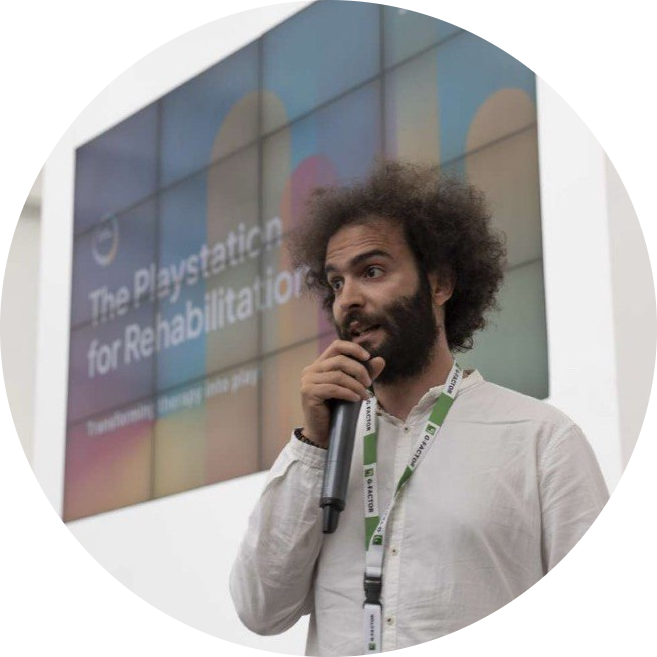
\includegraphics[width=2.8cm]{Pictures/Giovanni_pitch}
\end{minipage}
\vspace{0.1em}
}

\makeatletter
% the sender details are already in \clheader, so skip moderncv's own block
\@detailsfalse
% closing phrase, signature, name
\renewcommand*{\makeletterclosing}{%
  \@closing\\[0.6em]%
  
\includegraphics[height=1.2cm]{Pictures/sign_gt.jpg}\\[0.2em]%
  {\bfseries\@firstname~\@lastname}}
\makeatother


\begin{document}

\clheader{Product Researcher | Interviews, Usability Testing \& Synthesis}

\recipient{Ethos}{Expert Network}
\opening{Dear Ethos Team,}
\closing{Sincerely,}
\makelettertitle

I am applying for the Product Researcher opportunity to help train a language model on research documents, spreadsheets and slide decks. I am Head of Product and co-founder of Rehabilia Technologies, and for more than five years I have run customer and user research at CNR-STIIMA, the Italian National Research Council. Judging whether a findings deck or an interview synthesis actually helps a team decide is part of my daily work, so I would enjoy doing it for AI-generated ones.

I own studies from start to finish. I write the study protocol, run interviews and usability tests, collect questionnaire data, analyse it and turn it into findings that a team can act on. I have run studies with 16 blind participants for an indoor navigation system and with children with cerebral palsy for a rehabilitation game, which we published as a usability and acceptability pilot study in the \textit{Italian Journal of Pediatrics}. At Rehabilia, I lead discovery interviews with clinicians, patients and partners and ongoing field research with clinics, and I synthesise what I hear into problem statements, journey maps and product recommendations. Our device PhiCube reached a usability score of 85.8/100 (SUS) with 19 children, and in the preliminary results of a multicentre study across six Italian clinics, 55 children aged 4 to 17 rated every usability and acceptability item above 4 out of 5.

Most of my output is written: study protocols, reports, papers and presentations for clinicians, partners and funders, so I care about clear structure and precise wording. I also use Claude and Claude Code every day to draft, analyse and structure documents, and I hold Anthropic's certifications for both, so I know where model output tends to look polished but miss the point.

My research has been in healthcare and assistive technology rather than commercial software, and I have used standardised questionnaires more than custom survey instruments. The core skills are the same: planning a study, listening carefully and turning raw data into conclusions people can trust.

I am available to work 5 to 20 hours per week, remotely and on a flexible schedule, and I would welcome the chance to contribute.

\makeletterclosing

\end{document}
